
\section{Additional Results} \label{AppendixA}

\subsection{Logistic regression for assistance applications}


\begin{table}[htbp]
   \centering
   \caption{\label{ResultsLogit} Determinants of Assistance Application}
   \begin{tabular}{lc}
      \tabularnewline\midrule\midrule
      Dependent Variable:        & Applicant\\
      Model:                     & (1)\\
      \midrule \emph{Variables} &  \\
      (Intercept)                & -3.622\\
                                 & (3.723)\\
      Share of democratic voters & -0.8362$^{**}$\\
                                 & (0.3469)\\
      Median Income (logs)       & 0.2939\\
                                 & (0.3331)\\
      Poverty Rate               & 4.033$^{**}$\\
                                 & (1.575)\\
      Share of single mothers    & 4.068$^{***}$\\
                                 & (1.144)\\
      \midrule \emph{Fit statistics} &  \\
      Observations               & 2,882\\
      Squared Correlation        & 0.02306\\
      Pseudo R$^2$               & 0.01966\\
      BIC                        & 3,724.7\\
      \midrule\midrule\multicolumn{2}{l}{\emph{IID standard-errors in parentheses}}\\
      \multicolumn{2}{l}{\emph{Signif. Codes: ***: 0.01, **: 0.05, *: 0.1}}\\
   \end{tabular}
\end{table}




\subsection{Dynamic Treatment Effects}


\begin{table}[htbp]
   \centering
   \caption{\label{MainResultsMath} Results (Mathematics)}
   \begin{tabular}{lccccc}
      \tabularnewline\midrule\midrule
      Dependent Variables: & Overall         & Black           & Hispanic        & Female          & Econ. Disadv.\\
      Model:               & (1)             & (2)             & (3)             & (4)             & (5)\\
      \midrule \emph{Variables} &   &   &   &   &  \\
      Year$=$-5            & -0.0319$^{***}$ & -0.0593$^{***}$ & -0.0407$^{***}$ & -0.0243$^{***}$ & -0.0529$^{***}$\\
                           & (0.0039)        & (0.0059)        & (0.0062)        & (0.0042)        & (0.0042)\\
      Year$=$-4            & -0.0129$^{***}$ & -0.0195$^{***}$ & -0.0167$^{**}$  & -0.0088$^{**}$  & -0.0226$^{***}$\\
                           & (0.0041)        & (0.0061)        & (0.0066)        & (0.0044)        & (0.0044)\\
      Year$=$-3            & -0.0063$^{*}$   & -0.0214$^{***}$ & -0.0042         & -0.0056         & -0.0107$^{***}$\\
                           & (0.0037)        & (0.0055)        & (0.0058)        & (0.0039)        & (0.0039)\\
      Year$=$-2            & -0.0034         & -0.0099$^{**}$  & -0.0011         & -0.0017         & -0.0023\\
                           & (0.0032)        & (0.0050)        & (0.0051)        & (0.0034)        & (0.0035)\\
      Year$=$0             & -0.0064$^{**}$  & -0.0054         & -0.0024         & -0.0047         & -0.0049\\
                           & (0.0028)        & (0.0045)        & (0.0045)        & (0.0030)        & (0.0031)\\
      Year$=$1             & -0.0089$^{***}$ & -0.0041         & -0.0055         & -0.0054$^{*}$   & -0.0006\\
                           & (0.0030)        & (0.0049)        & (0.0049)        & (0.0032)        & (0.0032)\\
      Year$=$2             & -0.0064$^{**}$  & 0.0041          & -0.0018         & -0.0078$^{**}$  & 0.0011\\
                           & (0.0033)        & (0.0053)        & (0.0053)        & (0.0035)        & (0.0035)\\
      Year$=$3             & -0.0093$^{***}$ & -0.0077         & -0.0114$^{**}$  & -0.0141$^{***}$ & -0.0006\\
                           & (0.0034)        & (0.0056)        & (0.0055)        & (0.0036)        & (0.0036)\\
      Year$=$4             & -0.0145$^{***}$ & -0.0122$^{**}$  & -0.0132$^{**}$  & -0.0145$^{***}$ & -0.0057\\
                           & (0.0037)        & (0.0061)        & (0.0059)        & (0.0039)        & (0.0040)\\
      Year$=$5             & -0.0133$^{***}$ & -0.0138$^{*}$   & -0.0121$^{*}$   & -0.0159$^{***}$ & -0.0109$^{**}$\\
                           & (0.0041)        & (0.0073)        & (0.0068)        & (0.0044)        & (0.0045)\\
      Year$=$6             & -0.0049         & 0.0026          & 0.0012          & -0.0033         & -0.0072\\
                           & (0.0042)        & (0.0076)        & (0.0069)        & (0.0045)        & (0.0046)\\
      Year$=$7             & 0.0094$^{**}$   & 0.0083          & 0.0101          & 0.0104$^{**}$   & 0.0140$^{***}$\\
                           & (0.0048)        & (0.0084)        & (0.0080)        & (0.0051)        & (0.0052)\\
      Year$=$8             & 0.0124$^{**}$   & -0.0241$^{**}$  & 0.0044          & 0.0049          & 0.0027\\
                           & (0.0062)        & (0.0116)        & (0.0106)        & (0.0067)        & (0.0068)\\
      \midrule \emph{Fixed-effects} &   &   &   &   &  \\
      Year                 & Yes             & Yes             & Yes             & Yes             & Yes\\
      County               & Yes             & Yes             & Yes             & Yes             & Yes\\
      Grade                & Yes             & Yes             & Yes             & Yes             & Yes\\
      \midrule \emph{Fit statistics} &   &   &   &   &  \\
      Observations         & 158,110         & 65,729          & 70,149          & 150,052         & 147,520\\
      R$^2$                & 0.72280         & 0.56708         & 0.55530         & 0.67862         & 0.59956\\
      Within R$^2$         & 0.00354         & 0.00971         & 0.00380         & 0.00320         & 0.00630\\
      \midrule\midrule\multicolumn{6}{l}{\emph{IID standard-errors in parentheses}}\\
      \multicolumn{6}{l}{\emph{Signif. Codes: ***: 0.01, **: 0.05, *: 0.1}}\\
   \end{tabular}
\end{table}





\begin{table}[htbp]
   \centering
   \caption{\label{MainResultsRLA} Results (RLA)}
   \begin{tabular}{lccccc}
      \tabularnewline\midrule\midrule
      Dependent Variables: & Overall       & Black          & Hispanic     & Female                 & Econ. Disadv.\\
      Model:               & (1)           & (2)            & (3)          & (4)                    & (5)\\
      \midrule \emph{Variables} &   &   &   &   &  \\
      Year$=$-5            & -0.0031       & -0.0265$^{**}$ & -0.0202      & -0.0147                & -0.0247$^{***}$\\
                           & (0.0063)      & (0.0102)       & (0.0131)     & (0.0176)               & (0.0070)\\
      Year$=$-4            & 0.0067        & 0.0022         & 0.0001       & $-1.34\times 10^{-5}$ & 0.0047\\
                           & (0.0038)      & (0.0047)       & (0.0074)     & (0.0106)               & (0.0050)\\
      Year$=$-3            & 0.0068$^{**}$ & 0.0037         & 0.0108$^{*}$ & 0.0007                 & 0.0083$^{*}$\\
                           & (0.0030)      & (0.0028)       & (0.0053)     & (0.0077)               & (0.0041)\\
      Year$=$-2            & 0.0003        & -0.0012        & -0.0051      & -0.0007                & 0.0007\\
                           & (0.0016)      & (0.0021)       & (0.0029)     & (0.0032)               & (0.0025)\\
      Year$=$0             & 0.0006        & 0.0085$^{**}$  & 0.0016       & 0.0012                 & -0.0011\\
                           & (0.0022)      & (0.0037)       & (0.0031)     & (0.0026)               & (0.0032)\\
      Year$=$1             & 0.0003        & 0.0173$^{**}$  & 0.0108$^{*}$ & 0.0101                 & 0.0048\\
                           & (0.0039)      & (0.0067)       & (0.0058)     & (0.0064)               & (0.0056)\\
      Year$=$2             & 0.0031        & 0.0170$^{**}$  & 0.0059       & 0.0137                 & 0.0074\\
                           & (0.0048)      & (0.0058)       & (0.0076)     & (0.0097)               & (0.0064)\\
      Year$=$3             & 0.0043        & 0.0162         & 0.0085       & 0.0162                 & 0.0069\\
                           & (0.0053)      & (0.0102)       & (0.0096)     & (0.0125)               & (0.0070)\\
      Year$=$4             & 0.0038        & 0.0269$^{**}$  & 0.0142       & 0.0235                 & 0.0164$^{*}$\\
                           & (0.0067)      & (0.0119)       & (0.0131)     & (0.0152)               & (0.0074)\\
      Year$=$5             & 0.0131        & 0.0369$^{**}$  & 0.0215       & 0.0252                 & 0.0188$^{*}$\\
                           & (0.0079)      & (0.0142)       & (0.0152)     & (0.0206)               & (0.0099)\\
      Year$=$6             & 0.0135        & 0.0473$^{***}$ & 0.0290       & 0.0302                 & 0.0144\\
                           & (0.0099)      & (0.0137)       & (0.0192)     & (0.0233)               & (0.0108)\\
      Year$=$7             & 0.0237        & 0.0609$^{**}$  & 0.0403       & 0.0447                 & 0.0230\\
                           & (0.0135)      & (0.0207)       & (0.0232)     & (0.0268)               & (0.0139)\\
      Year$=$8             & 0.0234        & 0.0275         & 0.0162       & 0.0366                 & 0.0159\\
                           & (0.0167)      & (0.0240)       & (0.0286)     & (0.0293)               & (0.0201)\\
      \midrule \emph{Fixed-effects} &   &   &   &   &  \\
      Year                 & Yes           & Yes            & Yes          & Yes                    & Yes\\
      County               & Yes           & Yes            & Yes          & Yes                    & Yes\\
      Grade                & Yes           & Yes            & Yes          & Yes                    & Yes\\
      \midrule \emph{Fit statistics} &   &   &   &   &  \\
      Observations         & 169,246       & 71,155         & 74,154       & 160,296                & 157,873\\
      R$^2$                & 0.74510       & 0.59150        & 0.59889      & 0.71173                & 0.61003\\
      Within R$^2$         & 0.00353       & 0.00675        & 0.00612      & 0.00422                & 0.00395\\
      \midrule\midrule\multicolumn{6}{l}{\emph{Clustered (Cohort) standard-errors in parentheses}}\\
      \multicolumn{6}{l}{\emph{Signif. Codes: ***: 0.01, **: 0.05, *: 0.1}}\\
   \end{tabular}
\end{table}




\newpage

\section{Pre-Treatment Trends} \label{PreTrends}

Here we display plots of aggregated pre-treatment trends to justify the parallel trends assumption. Mean test scores are aggregated by cohort (year of first treatment) and relative time to treatment, and never treated units act as the control group. Figure \ref{PreTrendsMath} and \ref{PreTrendsRLA} show the results for mathematics and RLA respectively. We only display these plots for overall test scores and not for subgroups. However, the plots for the subgroups look very similar.


\begin{figure}[!h]
	\centering
	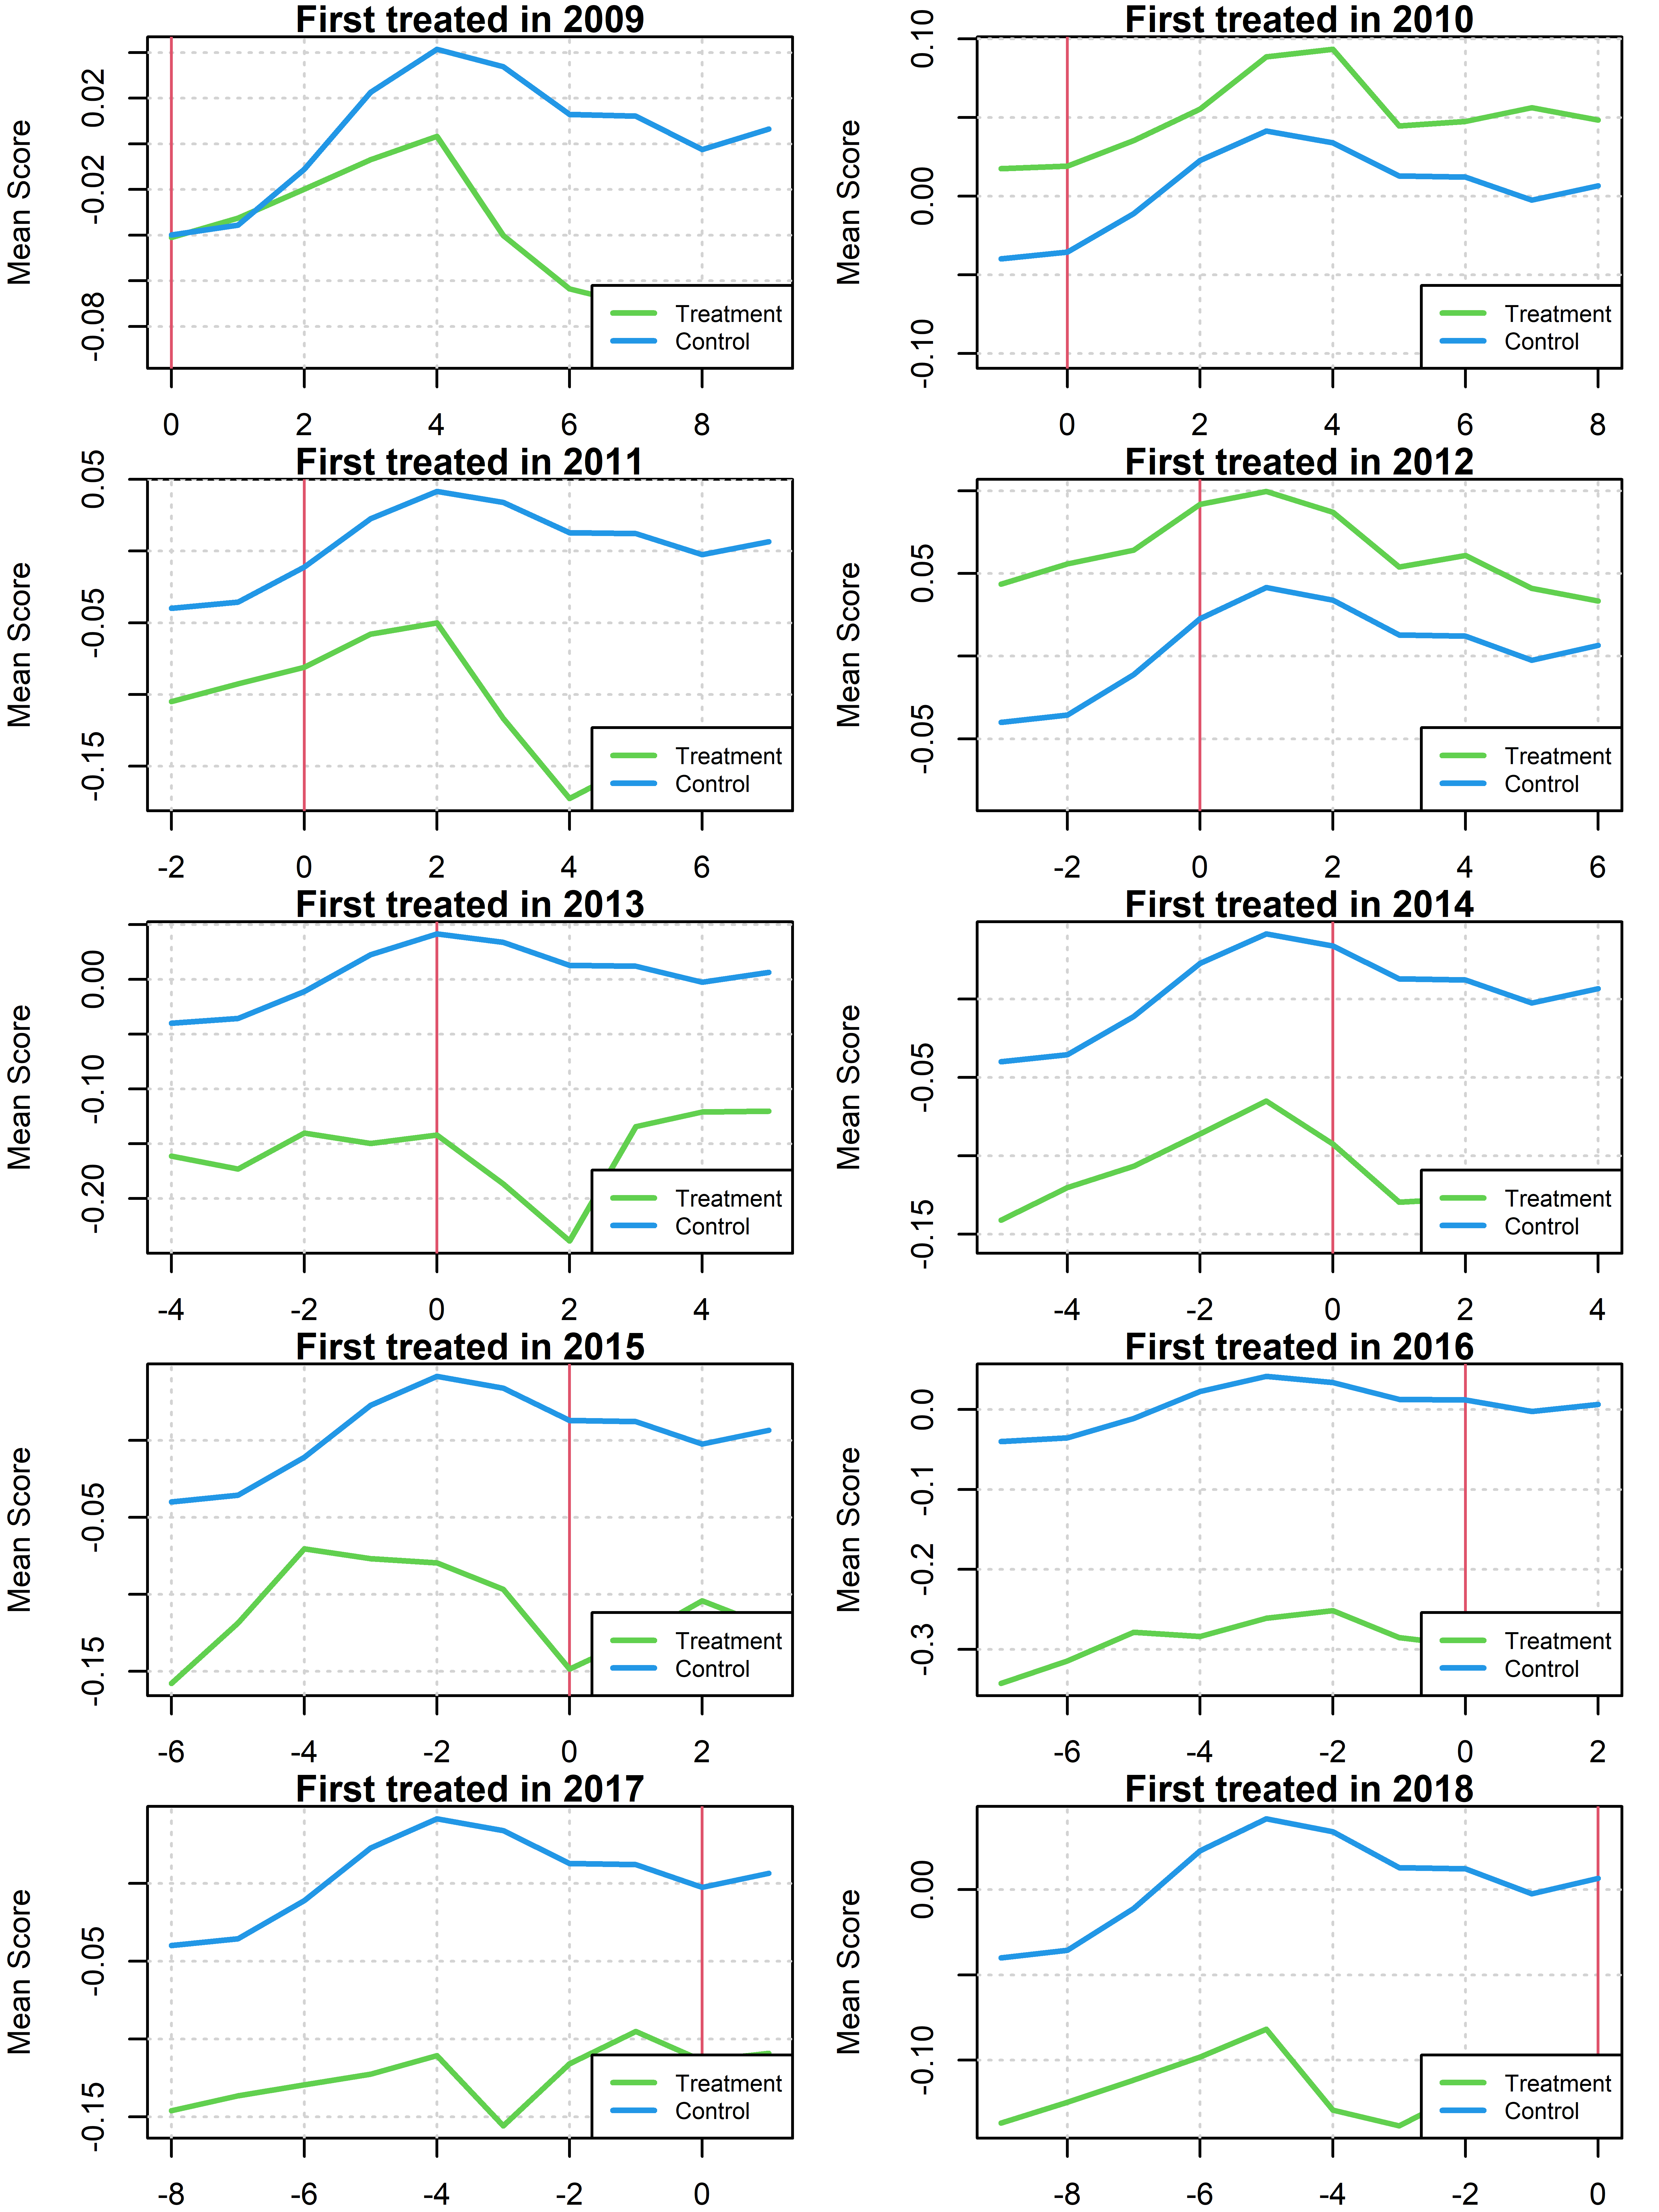
\includegraphics[scale=1]{"../Code & Data/ParTrendsPlotMathematics.png"}
	\caption{Pre trends for aggregated mean scores in mathematics}
	\label{PreTrendsMath}
\end{figure}

\begin{figure}[!h]
	\centering
	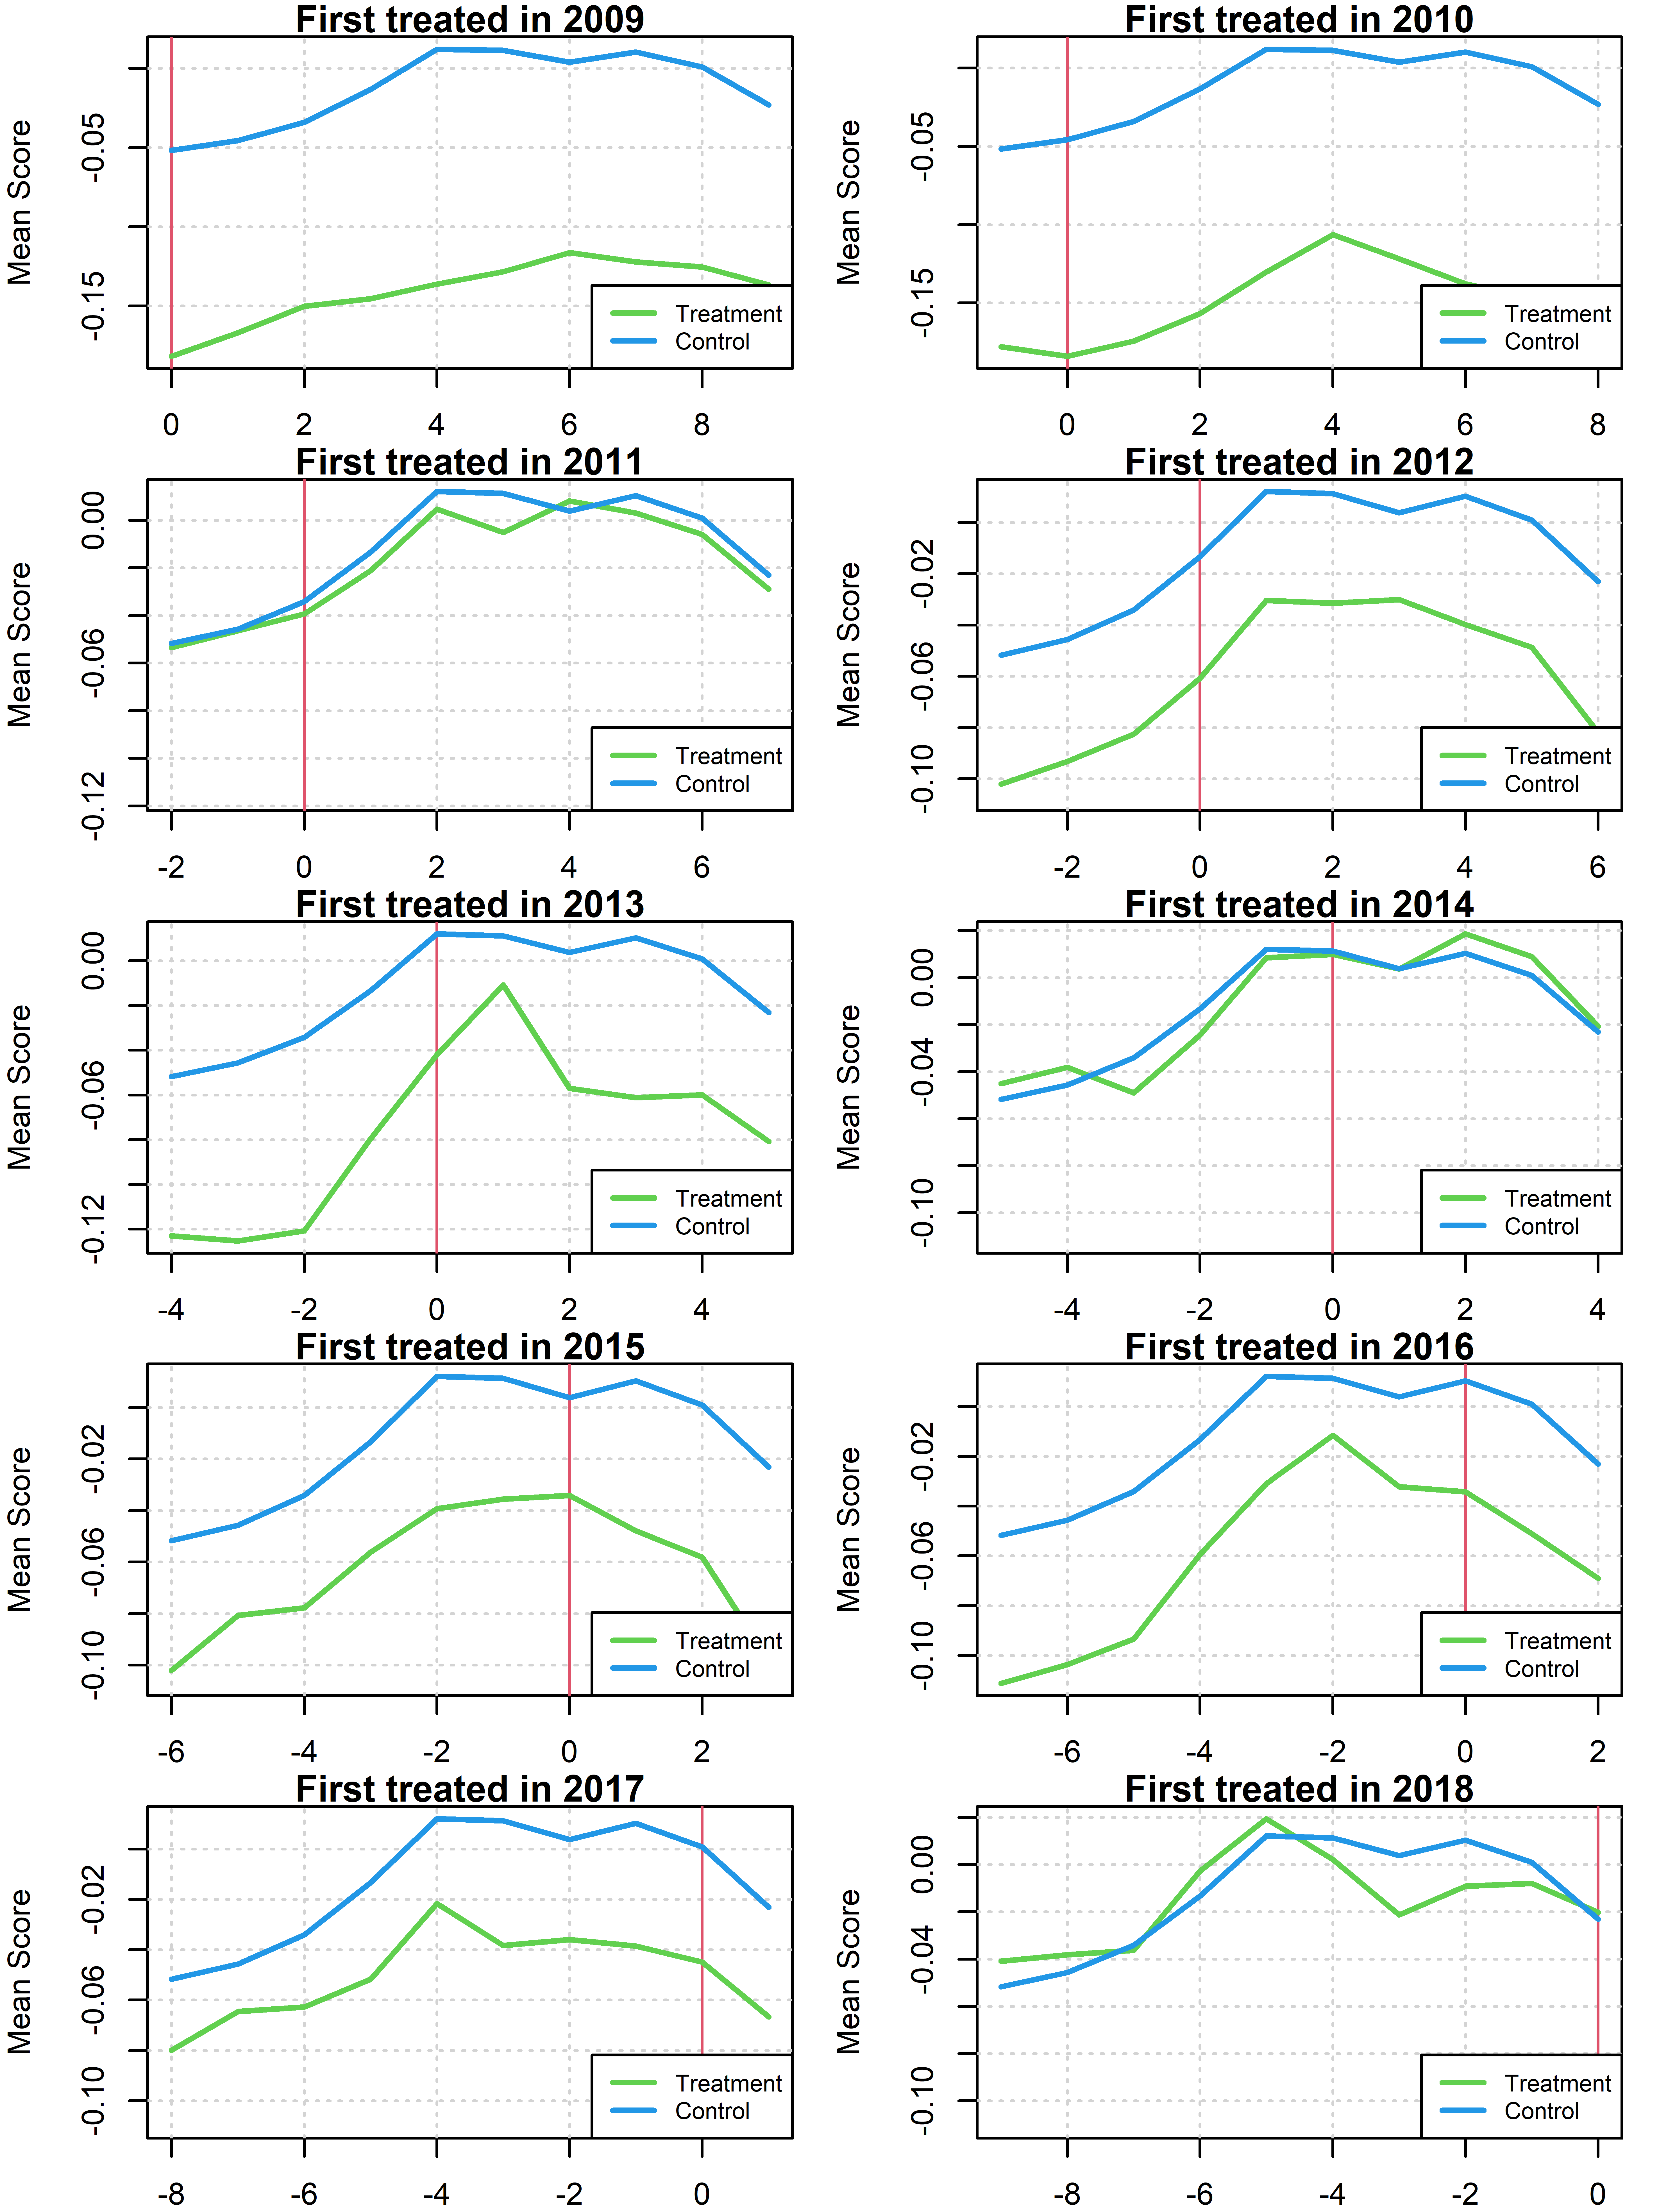
\includegraphics[scale=1]{"../Code & Data/ParTrendsPlotRLA.png"}
	\caption{Pre trends for aggregated mean scores in RLA}
	\label{PreTrendsRLA}
\end{figure}



